\section{Perils of disregard}
\label{sec:graph-importance}

Consider the proposals from the following fictitious scenarios: 
- Based on input from the public, the Department of Transportation (DOT) of  is considering implementing a new parking policy. 
This proposed policy would put in place pricing changes and parking restrictions that would discourage individuals from parking in the central business district. 
The DOT (and its constituents) believes that this policy would encourage people to use more active transportation modes (e.g: walking, biking, etc..).
- A certain DOT is considering constructing a streetcar (trolley, tram) line in a low/mid-income area in its jurisdiction.
Citing examples from other cities and countries, the DOT claims that the new streetcar line will create more transit oriented
developments and increase economic activity in the areas surrounding the proposed project. 

%% TODO: Present an example or two of real life project proposals?

Thinking more closely about these proposals, it is clear that they assume a causal relationship between the proposed project/policy and the desired goals. 
The DOT in question completed data analysis that allowed them to conclude that putting such policy or project in place would result in cause the desired output and achieve the desired goal.
In the presented scenarios, the DOT claims that implementing the new parking policy will cause an increase the share of 
active transportation modes in the central business district and constructing the proposed streetcar line will 
cause an increase more transit oriented developments and economic activity.

Policymakers base their analyses and conclusions on hypotheses or beliefs of how the world operates.
In other words, the data analysis is based on a certain belief about the data generating process.
Yet, policymakers often do not present their beliefs about such data generating process.
As a result, these proposals maintain an obscure representation of how the policy or project will achieve their desired goals. 

Directed Acyclic Graphs (DAGs) allow one to clearly encode their assumptions about the data generating process and the problem at hand.
Researchers and practitioners have made use of DAGs in fields such as epidemiology, scheduling, and network structures and have found them to be practical.

%% TODO: maybe insert some references of where DAGs were used?.

DAGs could show to be very useful in addressing transportation policy questions, similar to the ones presented above.
\citet{brathwaite_2018_causal} have proposed a framework illustrating how practitioners and researchers can use DAGs
 to answer such transportation modeling questions in a causal context.
\citet{brathwaite_2018_causal}, however, have not shown an empirical application of their framework and how it results
 in different conclusions when compared to traditional modeling approaches.

In this section, we will present an example illustrating the importance of using DAGs in transportation demand modeling efforts. 
More specifically, we will illustrate how different assumptions about the data generating process result in different conclusions.
We approach this exercise by building up on \citet{brathwaite_2018_causal} work by going through 
an empirical exercise of a simplified transportation modeling problem.
Before going any further, we would like to note that this example is for
illustrative purposes and does not reflect the complexities of a typical transportation choice modeling problem.

Let us assume that a company wants to reduce its workforce carbon footprint by moving its employees closer to their campus. 
This action could lead to more employees not driving to work.
We would like to forecast how such an intervention would change the share of employees driving to work.
We model this travel mode choice problem based on a dataset from \citet{brathwaite_asymmetric}.
This dataset is based on the 2012 California Household Travel Survey (CHTS).
The dataset contains approximately 4000 home-based school or work tours made by approximately 3850 individuals in the California Bay area.
Readers interested in a more detailed description of the dataset can refer to \citet{brathwaite_asymmetric}.
Our goal in this section is not to recover the causal effect of the proposed intervention.
We aim to only show how different DAGs would result in different conclusions about the impact of the proposed intervention.
For purposes of this exercise, we consider the Multinomial Logit model defined in \citet{brathwaite_asymmetric} as the true outcome generating process.

The systematic utility equations of the adopted multinomial logit model are specified as follows:

\[ U_{da} = \beta_{travel time} \times Travel Time + \beta_{cost per distance da} \times Cost per Distance_{da} + \beta_{autos}  \times Number of Autos \]
\[ U_{sr2} = ASC_{sr2} + \beta_{time drive} \times Travel Time + \beta_{cost per distance sr2} \times Cost per Distance_{sr2} + \beta_{autos}  \times Number of Autos + \beta_{cross bay} \times Cross Bay + \beta_{hh size} \times HH Size + \beta_{n kids hh} \times Number of kids \]
\[ U_{sr3+} = ASC_{sr3+} + \beta_{time drive} \times Travel Time + \beta_{cost per distance sr3+} \times Cost per Distance_{sr3+} + \beta_{autos}  \times Number of Autos + \beta_{cross bay} \times Cross Bay + \beta_{hh size} \times HH Size + \beta_{n kids hh} \times Number of kids \]
\[ U_{WTW} = ASC_{WTW} + \beta_{travel time transit} \times Travel Time + \beta_{travel cost} \times Travel Cost \]
\[ U_{DTW} = ASC_{DTW} + \beta_{travel time transit} \times Travel Time + \beta_{travel cost} \times Travel Cost \]
\[ U_{WTD} = ASC_{WTD} + \beta_{travel time transit} \times Travel Time + \beta_{travel cost} \times Travel Cost \]
\[ U_{Bike} = ASC_{Bike} + \beta_{travel distance bike} \times Travel Distance \]
\[ U_{Walk} = ASC_{Walk} + \beta_{travel distance walk} \times Travel Distance \]

We achieve our goal through a simulation exercise as follows:

1. We build a DAG (graph 1) where we assume with all explanatory variables independent of each other. 
2. We simulate data based on this graph and generate outcomes based the chosen multinomial logit model.
4. We predict outcomes based on the mode choice model.
3. We apply the do-operator \citet{pearl_causality_2000} to reduce the travel distance for all individuals in the dataset and emulate a company's decision to move its employees closer to campus.
4. We predict new outcomes based on the mode choice model.

5. We build a different DAG (graph 2) for each utility function based on assumptions of how explanatory variables interact and influence the outcome.
6. We use the data at hand to estimate the relationships between different variables outlined in graph 2 .
7. We simulate data for variables not affected by any other nodes in graph 2 and use the estimated relationships from step 6 to simulate the remaining explanatory variables.
8. We then use the choice model to simulate outcome choices based on data simulated for graph 2.
9. We apply the do-operator to reduce the travel distance for all individuals in the dataset  and emulate a company's decision to move its employees closer to campus.
10. We use the estimated relationships from step 6 to simulate all the explanatory variables in graph 2 (namely the variables affected by travel distance).
11. We use the estimated choice model to produce outcomes based on the simulated data from step 10.

We repeat this simulation process several times and recover the choice probability of all modes for all individuals.
For our purposes, we focus on car-centric modes (Drive alone, Shared ride with another person, 
and a shared ride with two or more individuals).
We compute the difference in mode choice probabilities from different models based on the two constructed DAGs.

Figure \ref{fig:IND_GRAPH} illustrates the DAG where all explanatory variables are independent of each other for each utility equation (graph1).

\begin{figure}
   \centering
   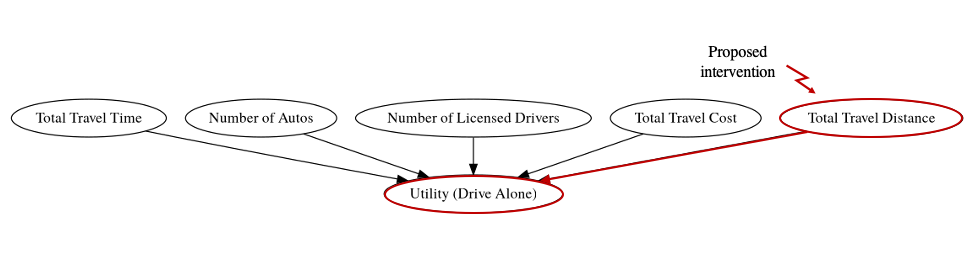
\includegraphics[width=0.5\textwidth]{Independent_graph.png}
   \caption{Causal Graph with Independent Covariates}
   \label{fig:IND_GRAPH}
\end{figure}

For our purposes, we assume that there are no latent variables.
The variables were chosen based on the specification of the MNL model outlined in \citet{brathwaite_asymmetric}.
We can describe the variables as follows:
- Total Travel Distance: is the total travel distance for individual i and mode j, for all available modes for individual i during trip t of tour l.
- Total Travel Cost: is the travel cost in dollars for individual i and mode j, for all available modes for individual i during trip t of tour l.
- Total travel time: is the travel time in minutes for individual i and mode j, for all available modes for individual i during trip t tour l.
- Number of Autos: is the number of automobiles owned by individual i's household.
- Number of Licensed Drivers: is the number of licensed drives in individual i's household.
- Number of Kids: is the number of kids in individual i's household.
- Cross-bay trip: is a binary variable indicating whether the trip t in tour l for individual i is a cross-bay trip.

Similarly, Figure \ref{fig:DA_causal_2} through \ref{fig:BIKE_causal_2} illustrate the causal graphs with "interacting" explanatory variables (graph 2).
Each of these graphs is based on the utility function of each mode in the multinomial logit model specified in \citet{brathwaite_asymmetric}.

\begin{figure}
   \centering
   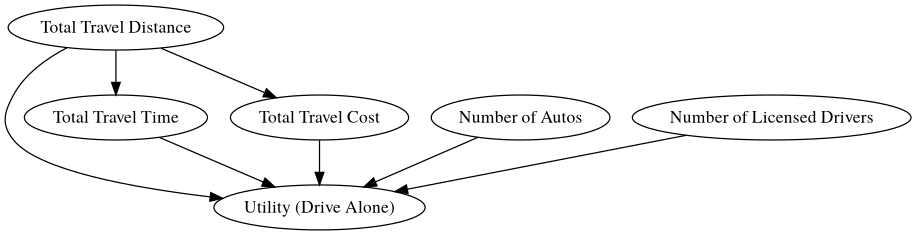
\includegraphics[width=0.5\textwidth]{DA_interacting_graph.png}
   \caption{Causal Graph for the Drive Alone Utility Function}
   \label{fig:DA_causal_2}
\end{figure}

\begin{figure}
   \centering
   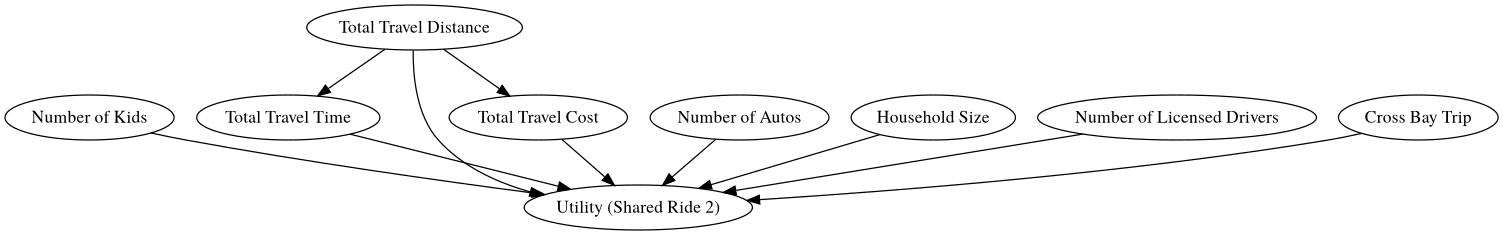
\includegraphics[width=0.5\textwidth]{SR2_interacting_graph.png}
   \caption{Causal Graph for the Shared Ride 2 Utility Function}
   \label{fig:SR2_causal_2}
\end{figure}

\begin{figure}
   \centering
   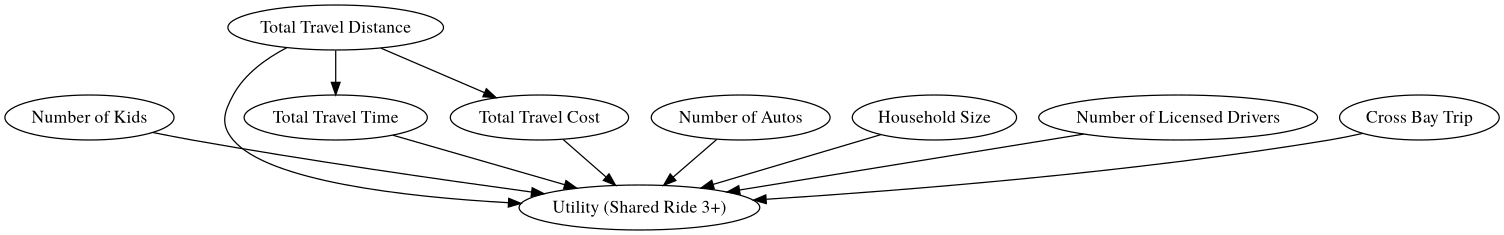
\includegraphics[width=0.5\textwidth]{SR3_interacting_graph.png}
   \caption{Causal Graph for the Shared Ride 3+ Utility Function}
   \label{fig:SR3_causal_2}
\end{figure}

\begin{figure}
   \centering
   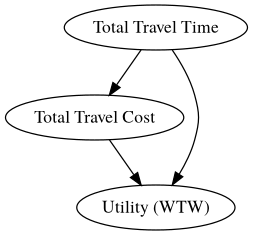
\includegraphics[width=0.5\textwidth]{WTW_interacting_graph.png}
   \caption{Causal Graph for the Walk-Transit-Walk Utility Function}
   \label{fig:WTW_causal_2}
\end{figure}

\begin{figure}
   \centering
   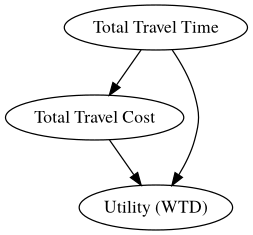
\includegraphics[width=0.5\textwidth]{WTD_interacting_graph.png}
   \caption{Causal Graph for the Walk-Transit-Drive Utility Function}
   \label{fig:WTD_causal_2}
\end{figure}

\begin{figure}
   \centering
   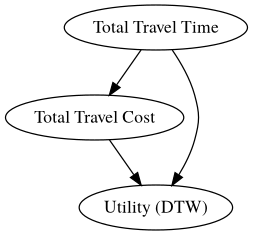
\includegraphics[width=0.5\textwidth]{DTW_interacting_graph.png}
   \caption{Causal Graph for the Drive-Transit-Walk Utility Function}
   \label{fig:DTW_causal_2}
\end{figure}

\begin{figure}
   \centering
   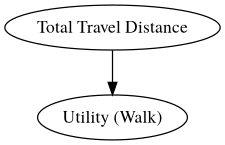
\includegraphics[width=0.5\textwidth]{WALK_interacting_graph.png}
   \caption{Causal Graph for the Shared Ride 3+ Utility Function}
   \label{fig:WALK_causal_2}
\end{figure}

\begin{figure}
   \centering
   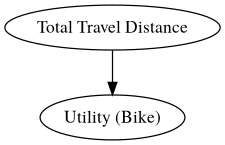
\includegraphics[width=0.5\textwidth]{BIKE_interacting_graph.png}
   \caption{Causal Graph for the Bike Utility Function}
   \label{fig:BIKE_causal_2}
\end{figure}

Each of these graphs is based on the utility function of each respective mode in the multinomial logit model estimated in \citet{brathwaite-asymmetric}.

We then plot histograms of the computed differences between the average probability of an individual
in our sample choosing a car centric mode before and after implementing a policy or intervention
aimed at reducing travel distance.
These differences are plotted under the two different assumptions about the data generating process illustrated in the causal graphs above.
Figure \ref{fig:histogram_probability} highlights the bias between the estimated probability of an average individual choosing a car centric mode.
This difference shows the importance of considering the data generating process when estimating transportation demand models aiming to forecast the impact of proposed policies.

\begin{figure}
   \centering
   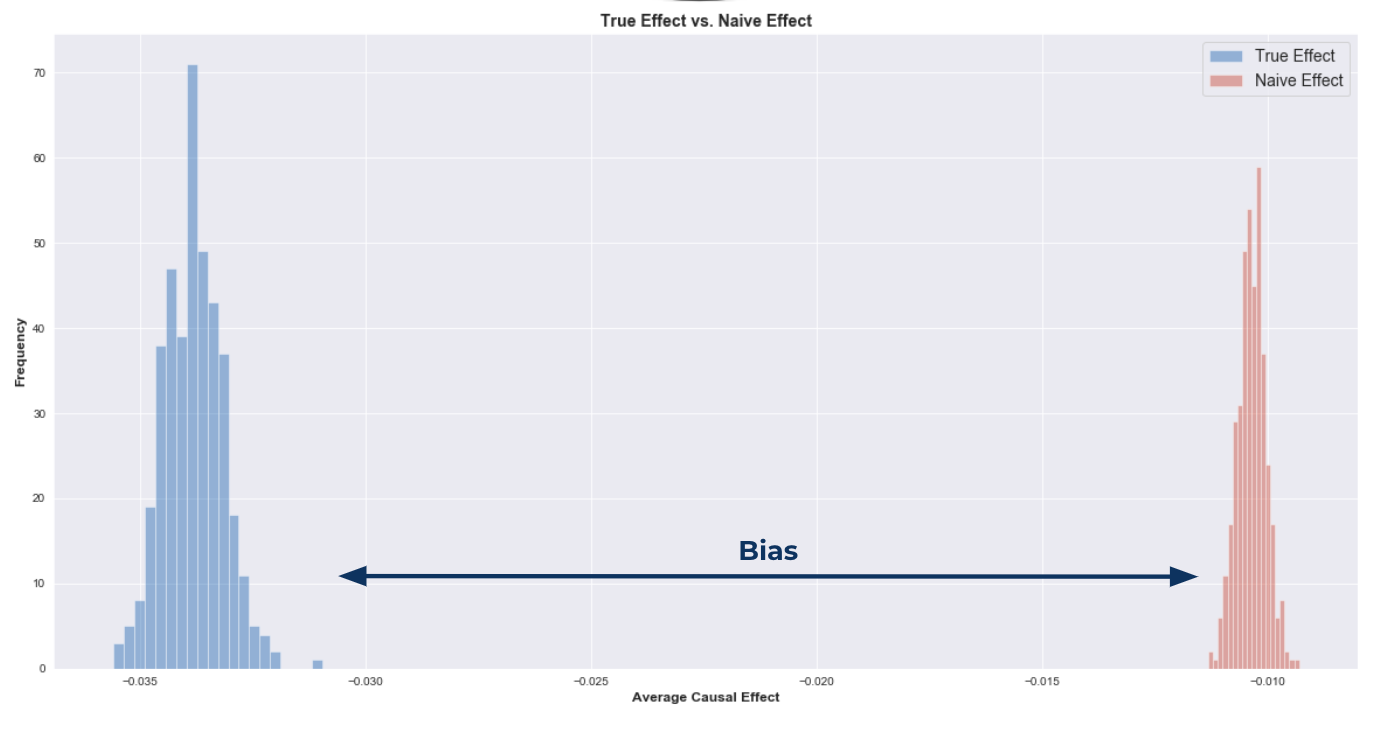
\includegraphics[width=0.5\textwidth]{histogram_selection_on_obs.png}
   \caption{Histograms of the probability of choosing Car Centric Modes under Different Data Generating processes.}
   \label{fig:histogram_probability}
\end{figure}

The data generating process might not be easily distinguishable in the majority of situations, mainly due to the complexity of the real world.
Therefore, constructing a causal graph that represents the data generating process as much as possible is not an easy task.
The following section explores this topic and includes some guidance on how to build and test causal graphs representing the researchers beliefs about the data generating process.